\documentclass{article}[18pt]
\usepackage{/home/sam/Documents/School_Notes/format}
\lhead{AS Level Physics - Waves}

%File specific Preamble
%Refraction settings
\usetikzlibrary{decorations.pathmorphing,arrows,shapes,positioning,decorations.markings,angles,quotes}
\tikzstyle arrowstyle=[scale=1]
\tikzstyle directed=[postaction={decorate,decoration={markings,
    mark=at position .65 with {\arrow[arrowstyle]{stealth}}}}]
\tikzstyle reverse directed=[postaction={decorate,decoration={markings,
    mark=at position .65 with {\arrowreversed[arrowstyle]{stealth};}}}]

\begin{document}
\begin{center}
\underline{\huge Refraction, Diffraction and interference}
\end{center}
\section{Interference}
\textbf{Coherence} - Waves with the same frequency and a constant phase difference\\
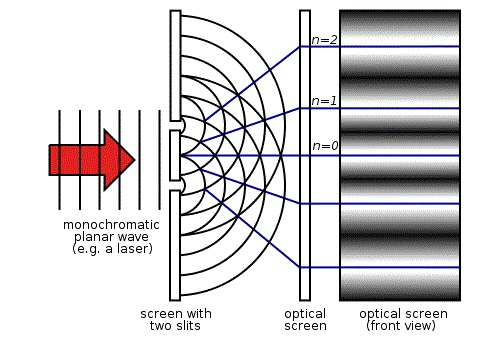
\includegraphics[width=10cm]{Interference.jpg}\\
When two of the same type of point meet they cause \textbf{reinforcement/constructive interference}\\
When a point meets with its opposite they cause \textbf{cancellation/destructive interference}
\section{Diffraction}
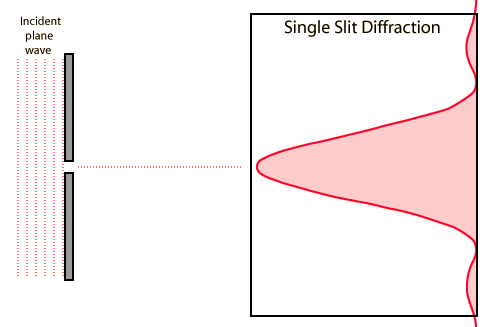
\includegraphics[width=7cm]{Diffraction.png}
\subsection{Diffraction of different colours}
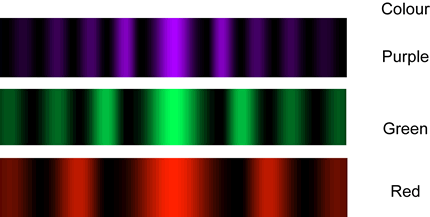
\includegraphics[width=7cm]{Diffraction_Colours.png}\\
Increasing wavelength:
\begin{itemize}
\item Central maxima becomes wider
\item Secondary maxima become wider apart
\end{itemize}
\newpage
\subsection{Deriving $n\lambda=d\sin\theta$}
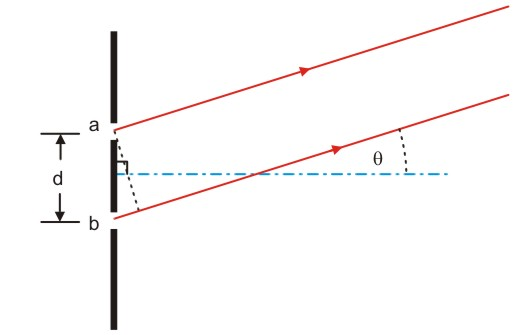
\includegraphics[width=7cm]{nlambda_1.png}\\
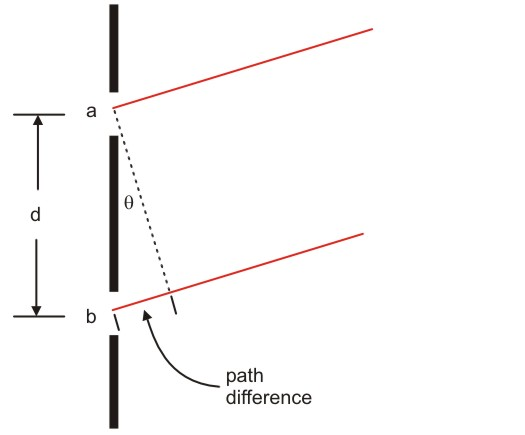
\includegraphics[width=7cm]{nlambda_2.png}\\
Path difference =$d\sin\theta$\\
$n\lambda=d\sin\theta$
\section{Refraction}
\subsection{Refraction at a plane surface}



\begin{figure}[h]
    \centering
    \begin{minipage}{0.28\textwidth}
        \centering
\begin{tikzpicture}[scale=0.5]

    % define coordinates
    \coordinate (O) at (0,0) ;
    \coordinate (A) at (0,4) ;
    \coordinate (B) at (0,-4) ;
    
    
    % media
    \fill[blue!25!,opacity=.3] (-4,0) rectangle (4,4);
    \fill[blue!60!,opacity=.3] (-4,0) rectangle (4,-4);
    \node[right] at (2,2) {Air};
    \node[left] at (3,-1.8) {Water};

    % axis
    \draw[dash pattern=on5pt off3pt] (A) -- (B) ;

    % rays
    \draw[red,ultra thick,reverse directed] (O) -- (240:4.63);
    \draw[blue,directed,ultra thick] (O) -- (45:4.24);

    % angles
;
    \node[] (a) at (240:4.63)  {};
    \node[] (c) at (270:4)  {};
    \node[] (b) at (270:0)  {};
    
    \node[] (d) at (45:4.24)  {};
    \node[] (e) at (90:4)  {};
    
    \draw pic["$\theta_1$",draw=black,-,angle eccentricity=1.2,angle radius=1.5cm] {angle=a--b--c};
    \draw pic["$\theta_2$",draw=black,-,angle eccentricity=1.2,angle radius=1.5cm] {angle=d--b--e};

    
   
\end{tikzpicture}
        \caption{Normal Refraction}
    \end{minipage}\hfill
    \begin{minipage}{0.28\textwidth}
        \centering
\begin{tikzpicture}[scale=0.5]

    % define coordinates
    \coordinate (O) at (0,0) ;
    \coordinate (A) at (0,4) ;
    \coordinate (B) at (0,-4) ;
    
    
    % media
    \fill[blue!25!,opacity=.3] (-4,0) rectangle (4,4);
    \fill[blue!60!,opacity=.3] (-4,0) rectangle (4,-4);
    \node[right] at (2,2) {Air};
    \node[left] at (3,-1.8) {Water};

    % axis
    \draw[dash pattern=on5pt off3pt] (A) -- (B) ;

    % rays
    \draw[red,ultra thick,reverse directed] (O) -- (230:4.63);
    \draw[blue,directed,ultra thick] (O) -- (0:4);

    % angles
;
    \node[] (a) at (230:4.63)  {};
    \node[] (c) at (270:4)  {};
    \node[] (b) at (270:0)  {};
    
    \draw pic["$\theta_C$",draw=black,-,angle eccentricity=1.2,angle radius=1.5cm] {angle=a--b--c};   
\end{tikzpicture}
        \caption{Critical angle}
    \end{minipage}\hfill
    \begin{minipage}{0.28\textwidth}
        \centering
\begin{tikzpicture}[scale=0.5]

    % define coordinates
    \coordinate (O) at (0,0) ;
    \coordinate (A) at (0,4) ;
    \coordinate (B) at (0,-4) ;
    
    
    % media
    \fill[blue!25!,opacity=.3] (-4,0) rectangle (4,4);
    \fill[blue!60!,opacity=.3] (-4,0) rectangle (4,-4);
    \node[right] at (2,2) {Air};
    \node[left] at (-1.8,-3) {Water};

    % axis
    \draw[dash pattern=on5pt off3pt] (A) -- (B) ;

    % rays
    \draw[red,ultra thick,reverse directed] (O) -- (210:4.63);
    \draw[blue,directed,ultra thick] (O) -- (330:4.63);

    % angles
;
    \node[] (a) at (210:4.63)  {};
    \node[] (c) at (270:4)  {};
    \node[] (b) at (270:0)  {};
    
    \node[] (d) at (330:4.24)  {};
    \node[] (e) at (270:4)  {};
    
    \draw pic["$\theta_1$",draw=black,-,angle eccentricity=1.2,angle radius=1cm] {angle=a--b--c};
    \draw pic["$\theta_2$",draw=black,-,angle eccentricity=1.2,angle radius=1cm] {angle=e--b--d};

    
   
\end{tikzpicture}
        \caption{Total internal reflection}
    \end{minipage}
\end{figure}
The angle is measured from the normal to the ray\\
After the angle reaches the critical angle the ray will undergo \textbf{total internal reflection}
\subsection{Fibre Optics}
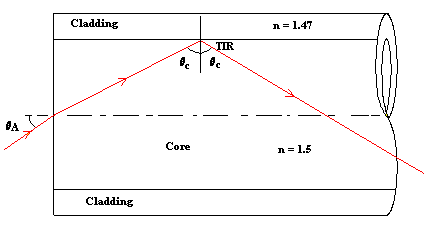
\includegraphics[width=7cm]{Fibre_Optic_1.png}\\
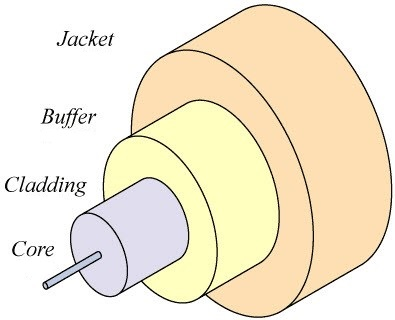
\includegraphics[width=7cm]{Fibre_Optic_2.jpg}\\
\subsubsection{Modal Dispersion}
Waves entering the fibre at different angles will reflect differently and so will have different path lengths
\subsubsection{Material Dispersion}
Different wavelengths of light enter the same but refract differently, causing a difference in path length





\end{document}
